\documentclass[../../index.tex]{subfiles}

\begin{document}
\chapter{$\tau$ decays into hadrons}
\begin{equation}
  R_\tau = \frac{\Gamma(\tau \to \nu_\tau + \text{Hadrons})}{\Gamma(\tau \to \nu_\tau e^+ e^-)}
\end{equation}

in terms of V/A, S/P \cite{Broadhurst1975}
\begin{equation}
  \begin{split}
    \Pi^{\mu\nu}(q^2) &= (q^\mu q^\nu - q^2 g^{\mu\nu}) \Pi^{V,A}(q^2) + \frac{g^{\mu\nu}}{q^2} (m_i \mp m_j)\Pi^{S,P}(q^2) \\
    &+ g^{\mu\nu}\frac{(m_i \mp m_j)}{q^2} [ \langle \anti{q}_i q_i \rangle \mp \langle \anti{q}_j q_j \rangle]
  \end{split}
\end{equation}

\begin{equation}
  q_\mu q_\nu \Pi^{\mu\nu}(q^2) = (m_i \mp m_j)^2 \Pi^{S,P}(q^2) + (m_i \mp m_j)[\langle \anti{q}_i q_i \rangle \mp \langle \anti{q}_j q_j \rangle]
\end{equation}

in terms of T and L
\begin{equation}
  (q^\mu q^\nu - g^{\mu\nu}q^2) \Pi^{(T)}(q^2) + q^\mu q^\nu \Pi^{(L)}(q^2)
\end{equation}

\begin{equation}
  q_\mu q_\nu \Pi^{\mu\nu}(q^2) = q^4 \Pi^{(L)}(q^2) = s^2 \Pi^{(L)}(s),
\end{equation}
where $s \equiv q^2$

relation L and S,P
\begin{equation}
  s^2 \Pi^{(L)}(s) = (m_i \mp m_j)^2 \Pi^{(S,P)}(s) + (m_i \mp m_j)[ \langle \anti{q}_i q_i \rangle \mp \langle \anti{q}_j q_j \rangle]
\end{equation}

need relation T and V,A
\begin{equation}
  \begin{split}
    \Pi^{\mu\nu}(s) &= \underbrace{(q^\mu q^\nu - g^{\mu\nu}q^2)\Pi^{(T)}(s) + (q^\mu q^\nu - g^{\mu\nu} q^2)\Pi^{(L)}(s)}_{=(q^\mu q^\nu - g^{\mu\nu} q^2) \Pi^{(T+L)}(s)} + \frac{g^{\mu\nu}s^2}{q^2}\Pi^{(L)}(s)
  \end{split} 
\end{equation}
where $\Pi^{(T+L)}(s) \equiv \Pi^{(T)}(s) + \Pi^{(L)}(s)$
\begin{equation}
  \Pi^{(V,A)}(s) = \Pi^{(T)}(s) + \Pi^{(L)} = \Pi^{(T+L)}
\end{equation}

\begin{equation}
  q_\mu q_nu
\end{equation}

The theoretical expression of the hadronic $\tau$-decay ratio was first derived
by \cite{Tsai1971} (using current algebra, a more recent derivation making use
of the *optical theorem* can be taken from \cite{Schwab2002}):
\begin{equation}
  \label{eq:hadronicTauDecayRatio}
  R_\tau = 12 \pi \int_0^{m_\tau} = \frac{\dif s}{m_\tau^2}
  \left( 1 - \frac{s}{m_\tau^2} \right)
  \left[ \left( 1 + 2 \frac{s}{m_\tau^2} \right) \Ima \Pi^{(T)}(s) + \Ima \Pi^{(L)} \right].
\end{equation}
$R_\tau$ introduces a problematic integral over the real axis of $\Pi(s)$ from $0$ up to
$m_\tau$. The integral is problematic for two reasons:
\begin{itemize}
  \item The \textit{perturbative Quantum Chromodynamcs} (\textbf{pQCD}) and the OPE breaks down for low
    energies (over which we have to integrate).
  \item The positive euclidean axis of $\Pi(s)$ has a discontinuity cut and can
    theoretically not be evaluated.
\end{itemize}
To literally circunvent these issues we make use of \textit{Cauchy's Theorem}
\begin{equation}
  \int_{\mathcal{C}} f(z) \dif z = 0,
\end{equation}
where $f(z)$ is an analytic function on a closed contour $\mathcal{C}$.

In our case we have to deal with the two-point correlator $\Pi(s)$, which is analytic
except for the positive real axis (with which we will deal with to a later
point\footnote{To not evaluate $\Pi(s)$ at the positive real axis we have to
  introduce \textit{pinched weights}. The \textit{pinched weights} vanish for $s
  \to m_\tau$.}) Consequently, to rewrite we can rewrite the definite integral of
\cref{eq:hadronicTauDecayRatio} into a contour integral over a closed circle
with
radius $m_\tau^2$. The closed contour consists of four line integrals,
which have been visualized in \cref{fig:rTauCauchysTheorem}. Summing over the
four line integrals, performing a \textit{analytic continuation} of the
two-point correlator $\Pi(s) \to \Pi(s + i \epsilon)$ and finally taking the
limit of $\epsilon \to 0$ gives us the needed relation between
\cref{eq:hadronicTauDecayRatio} and the closed contour:
\begin{equation}
  \begin{split}
  \oint_{s=m_\tau} \Pi(s) &= \int_0^{m_\tau} \Pi(s + i \epsilon) + \int_{\mathcal{C}_2}\Pi(s) \dif s + \int_{m_\tau}^0 \Pi(s - i \epsilon) \dif s + \int_{\mathcal{C}_4} \Pi(s) \dif s \\
  &= \int_0^{m_\tau} \Pi(s+i \epsilon) - \Pi(s - i \epsilon) \dif s  + \int_{\mathcal{C}_2}\Pi(s) \dif s + \int_{\mathcal{C}_4} \Pi(s) \dif s \\
  &= \int_0^{m_\tau} \Pi(s + i \epsilon) - \overline{\Pi(s + i \epsilon)} + \int_{\mathcal{C}_2}\Pi(s) \dif s + \int_{\mathcal{C}_4} \Pi(s) \dif s \\
  &\overset{\lim \epsilon \to 0}{=} 2 i \int_0^{m_\tau} \Ima \Pi(s) \dif s + \oint_{s=m_\tau} \Pi(s) \dif s
  \end{split}
\end{equation}
where we made use of $\Pi(z) = \overline{\Pi(\overline z)}$ (due to $\Pi(s)$ is analytic) and
$\Pi(z) - \overline{\Pi(z)} = 2 i \Ima \Pi(z)$. The result can be rewritten in a
more intuitive form, which we also visualized in \cref{fig:rTauCauchysTheorem}
\begin{equation}
  \label{eq:correlatorContourIntegral}
  \int_0^{m_\tau} \Pi(s) \dif s = \frac{i}{2} \oint_{s=m_\tau} \Pi(s) \dif s
\end{equation}
\begin{figure}
  \centering
  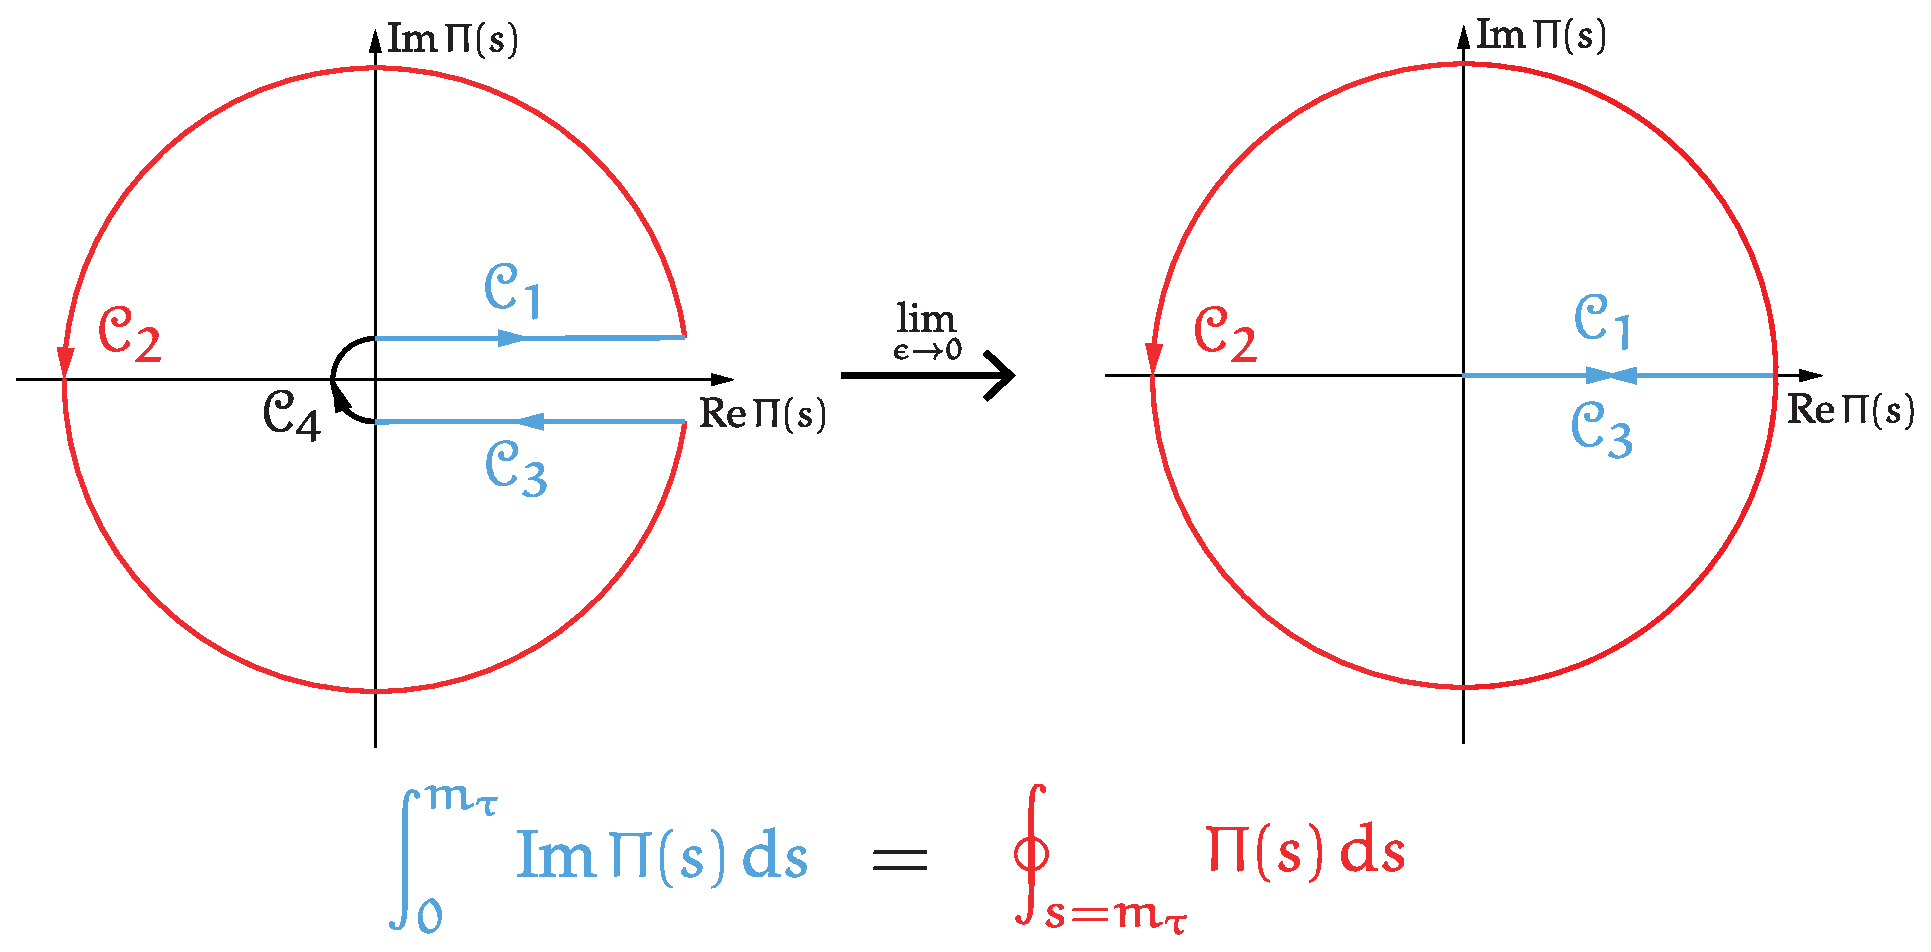
\includegraphics[width=0.8\textwidth]{./images/rTauCauchysTheorem.eps}
  \caption{Visualization of the usage of Cauchy's theorem to transform
    \cref{eq:hadronicTauDecayRatio} into a closed contour integral over a circle
  of radius $m_\tau^2$.}
  \label{fig:rTauCauchysTheorem}
\end{figure}
Finally combining \cref{eq:correlatorContourIntegral} with
\cref{eq:hadronicTauDecayRatio} we get
\begin{equation}
  R_\tau = 6 \pi i \oint_{s=m_\tau} \frac{\dif s}{m_\tau^2}
  \left( 1 - \frac{s}{m_\tau^2} \right)
  \left[ \left( 1 + 2 \frac{s}{m_\tau^2} \right) \Pi^{(T)}(s) + \Pi^{(L)} \right]
\end{equation}
for the hadronic $\tau$-decay ratio.

The contour integral obtained is an import result as we can now theoretically
evaluate the hadronic $\tau$-decay ratio sufficiently large energy scales
($m_\tau \approx \SI{1.78}{\mega\electronvolt}$) at which
$\alpha_s(m_\tau)\approx 0.33$ \cite{Pich2016} is tolerable heigh for applying
perturbation theory and the OPE. Obviously we would benefit from a contour integral over a
bigger circunference, but $\tau$-decays are limited by the $m_\tau$.
Nevertheless there are promising $e^+e^-$ annihilation data, which yields
valuable R-ratio values up to $\SI{2}{\giga\electronvolt}$
\cite{Boito2018}\cite{Keshavarzi2018}.

It is convenient to rewrite the 

\begin{equation}
  \Pi^{(L+T)} = \Pi^{(L)} + \Pi^{(T)}
\end{equation}

\begin{equation}
  R_\tau = 6 \pi i \oint_{\abs{s}=m_\tau} \frac{\dif s}{m_\tau^2} \left( 1 - \frac{s}{m_\tau^2} \right)^2 \left[ \left( 1 + 2 \frac{s}{m_\tau^2} \right) \Pi^{(L+T)}(s) - \left( \frac{2 s}{m_\tau^2} \right) \Pi^{(L)}(s) \right]
\end{equation}
\begin{equation}
  D^{(L+T)}(s) \equiv -s \od{}{s} \Pi^{(L+T)}(s), \qquad D^{(L)}(s) \equiv \frac{s}{m_\tau^2} \od{}{s} (s \Pi^{(L)}(s))
\end{equation}
Integration by parts
\begin{equation}
  \int_a^b u(x) V(x) \dif x = \left[ U(x) V(x) \right]_a^b - \int_a^b U(x) v(x) \dif x
\end{equation}
\begin{equation}
  \begin{split}
    R_\tau^{(1)} &= \frac{6 \pi i}{m_\tau^2} \oint_{\abs{s}=m_\tau^2}\underbrace{\left( 1 - \frac{s}{m_\tau^2} \right)^2 \left( 1 + 2 \frac{s}{m_\tau^2} \right)}_{=u(x)} \underbrace{ \vphantom{\left( \frac{s}{m_\tau^2} \right)} \Pi^{(L+T)}(s)}_{=V(x)} \\
    &= \frac{6 \pi i}{m_\tau^2} \left\{  \left[ -\frac{m_\tau^2}{2} \left( 1 - \frac{s}{m_\tau^2} \right)^3 \left( 1 + \frac{s}{m_\tau^2} \right) \Pi^{(L+T)}(s) \right]_{\abs{s}=m_\tau^2} \right. \\
    &\quad+ \oint_{\abs{s}=m_\tau^2} \underbrace{-\frac{m_\tau^2}{2} \left( 1 - \frac{s}{m_\tau^2} \right)^3 \left( 1 + \frac{s}{m_\tau^2} \right)}_{=U(x)} \underbrace{\vphantom{\left( \frac{1}{m_\tau^2} \right)}\od{}{s} \Pi^{(L+T)}(s)}_{=v(x)} \left. \vphantom{\left[ \left( \frac{1}{m_\tau^2} \right) \right]} \right\} \\
    &= -3 \pi i \oint_{\abs{s}=m_\tau^2s} \frac{\dif s}{s} \left( 1 - \frac{s}{m_\tau^2} \right)^3 \left( 1 + \frac{s}{m_\tau^2} \right) \od{}{s} D^{(L+T)}
  \end{split}
\end{equation}
where we fixed the integration constant to $C=-\frac{m_\tau^2}{2}$ in the second
line and left the antiderivatives contained in the squared brackets untouched.
Parametrizing the expression in the squared brackets
\begin{equation}
    \left[ -\frac{m_\tau^2}{2} \left( 1 - e^{-i \phi} \right)^3 \left( 1 + e^{-i \phi} \right) \Pi^{(L+T)}(m_\tau^2 e^{-i \phi}) \right]_0^{2\pi} = 0
\end{equation}
where $s \to m_\tau^2 e^{-i \phi}$ and $(1 - e^{-i \cdot 0}) = (1 - e^{-i \cdot 2 \pi})
= 0$.

\begin{equation}
  \begin{split}
    R_\tau^{(2)} &= \oint_{\abs{s}=m_\tau^2} \dif s \left( 1 - \frac{s}{m_\tau^2} \right)^2 \left( - \frac{2 s}{m_\tau^2} \right) \Pi^{(L)}(s) \\
    &= - 4 \pi i \oint \frac{\dif s}{s} \left( 1 - \frac{s}{m_\tau^2} \right)^3 D^{(L)}(s)
  \end{split}
\end{equation}

\begin{equation}
  R_\tau = - \pi i \oint_{\abs{s}=m_\tau^2} \frac{\dif}{s} \left( 1 - \frac{s}{m_\tau^2} \right)^3 \left[ 3 \left( 1 + \frac{s}{m_\tau^2} D^{(L+T)}(s) + 4 D^{(L)}(s) \right) \right]
\end{equation}

\begin{equation}
  R_\tau = - \pi i \oint_{\abs{s}=m_\tau^2} \frac{\dif}{x} (1 - x)^3 \left( 3 (1 + x) D^{(L+T)}(s) + 4 D^{(L)}(s)  \right),
\end{equation}
where $x=s/m_\tau^2$.
\end{document}